\documentclass[10pt,a4paper]{article}

\usepackage[a4paper,hmargin=2.5cm,vmargin=3cm] {geometry}
\usepackage{fix-cm}
\usepackage{amsmath,amssymb}
\usepackage{tikz}
\usepackage{graphicx}
\usepackage[polish,english]{babel}
\usepackage[T1]{fontenc}
\usepackage[utf8]{inputenc}
\usepackage{url}
\usepackage{verbatim}
\usepackage{color}
\usepackage{ae}
\usepackage[ruled]{algorithm}
\usepackage{algorithmicx}
\usepackage{algpseudocode}
\usepackage[breaklinks]{hyperref}
\usepackage[polish,english]{babel}
\usepackage{multirow}
\usepackage{listings}

\newtheorem{theorem}{Theorem}
\newtheorem{lemma}{Lemma}

\definecolor{myRed}{rgb}{0.9,0.3,0.1}
\newcommand{\pawel}[1]{\noindent\colorbox{myRed}{Pawel: #1}}
\definecolor{myYellow}{rgb}{0.99,0.99,0.05}
\newcommand{\jarek}[1]{\noindent\colorbox{myYellow}{Jarek: #1}}
\newcommand{\todo}[1]{\noindent\colorbox{myRed}{TODO: #1}}

\newcommand{\Oh}{\mathcal{O}}

\begin{document}

%%%%%%%%%%%%%%%%%%%%%%%%%%%%%%%%%%%%%%%%%%%%%%%%%%

\pagenumbering{roman}

\topmargin-20pt
\oddsidemargin0pt
\evensidemargin0pt
\textheight660pt
\textwidth445pt

\selectlanguage{polish}
\begin{titlepage}
\Large

\begin{center}

\textbf{\large%
Uniwersytet Wrocławski\\
Wydział Matematyki i Informatyki\\
Instytut Informatyki}


\vspace{4cm}
Jarosław Gomułka [DRAFT]

\vspace{0.5cm}
\textbf{%\normalsize%
Shuffla: fast and scalable full-text search engine}

\end{center}

\vspace{7cm}
\begin{flushright}
\begin{minipage}[c]{6.2cm}
  Praca magisterska\\
  napisana pod kierunkiem\\
  dr. Pawła Gawrychowskiego
\end{minipage}
\end{flushright}

\vfill

\begin{center}
 Wrocław 2012
\end{center}

\newpage

\end{titlepage}

\newpage

\thispagestyle{empty}

\Large

~\vfill
Oświadczam, że pracę magisterską wykonałem samodzielnie i zgłaszam ją do oceny.

\vspace{2cm}
Data: \dotfill\quad Podpis autora pracy: \dotfill


\vspace{4cm}
Oświadczam, że praca jest gotowa do oceny przez recenzenta.

\vspace{2cm}
Data: \dotfill\quad Podpis opiekuna pracy: \dotfill

\normalsize

\restoregeometry
%%%%%%%%%%%%%%%%%%%%%%%%%%%%%%%%%%%%%%%%%%%%%%%%%%

\newpage
\thispagestyle{empty}

\begin{abstract}
Celem tej pracy jest stworzenie efektywnego i skalowalnego narzędzia do dokładnego przeszukiwania zbioru użytkowników dużego portalu społecznościowego. Rrzechowane dane to imię, nazwisko, wiek, oraz miejsce zamieszkania.

Użytkownik portalu może wyszukiwać innych użytkowników poprzez:
\bigskip
\begin{enumerate}
\item{podanie imienia (jego prefiksu lub podsłowa),}
\item{podanie nazwiska (jego prefiksu lub podsłowa),}
\item{podanie wieku (dokładnie bądź przez określenie dolnej i górnej granicy),}
\item{podanie miejsca zamieszkania (jego prefiksu lub podsłowa).}
\end{enumerate}

\bigskip

Kolejnym założeniem jest konieczność personalizacji wyników wyszukiwania. Na przykładu użytkownik z San Francisco szukający Jane powinien dostać w pierwszej kolejności osoby o imieniu Jane z San Francisco, następnie osoby z Kaliforni, Stanów Zjednoczonych, a dopiero na samym końcu z innych części świata.

Jednym z możliwych rozwiązań tak postawionego problemu jest zastosowanie jednej z popularnych relacyjnych baz danych. Inną możliwością jest użycie wyszukiwarki tekstowej takiej jak Apache Solr czy Sphinx Search. Jeszcze innym pomysłem jest zaimplementowanie własnego narzędzia. Celem tej pracy jest przedstawienie Shuffli, wyspecjalizowanej wyszukiwarki stworzonej przeze mnie z myślą o tym konkretnym problemie. Oprócz przedstawienia architektury i szczegółów implementacji, porównam jej efektywność z PostgreSQL, Apache Solr, Sphinx Search.

\bigskip
Pracuję nad portalem nk.pl (który jest największym polskim portalem społecznościowym) od początku roku 2011. W sierpniu 2011 roku zostało mi powierzone rozwiązanie tego problemu.

\bigskip
\noindent \textbf{Słowa kluczowe:} bazy danych, nosql
\end{abstract}

\selectlanguage{english}
%%%%%%%%%%%%%%%%%%%%%%%%%%%%%%%%%%%%%%%%%%%%%%%%%%


\title{Shuffla: fast and scalable full-text search engine}
\author{Jarosław Gomułka}

\maketitle

\begin{abstract}
Given a list of people (their first name, last name, age, home town) we want to provide high-available, scalable and very fast solution that can search through such data.
User can narrow search results by:

\bigskip
\begin{enumerate}
\item{defining first name (its prefix or substring)}
\item{defining last name (its prefix or substring)}
\item{narrowing age (user can provide lower or/and upper bound for age)}
\item{defining city (its prefix or substring)}
\end{enumerate}

\bigskip
It would be great if results could be personalized. For example, if user from San Francisco is looking for Jane, top results should show Jane's from San Francisco, then Jane's from California, then rest of U.S. One of possible solution is to use relational database. Other solution is to use full-text search engine like Apache Solr or Sphinx Search. Another solution is to develop very own search engine dedicated to solving such task. In this paper I will describe Shuffla, full-text search engine created by me. I will compare it to Sphinx, Solr, PostgreSQL. 

\bigskip
I'm working on nk.pl (which is biggest polish social networking website) since the beginning of 2011. In August 2011 I was appointed to solve task described above. 

\bigskip
\noindent \textbf{Keywords:} database, nosql
\end{abstract}

\pagenumbering{arabic}
%%%%%%%%%%%%%%%%%%%%%%%%%%%%%%%%%%%%%%%%%%%%%%%%%%

\section{Problem definition}

Lets define table definition by combination of
\begin{enumerate}
\item table name
\item list of pairs <column name, type of column>
\end{enumerate}
Type of column can be either string or number

\subsection{Selecting data}
There are different possible conditions for different types. Possible conditions for numbers are comparisons, inequalities and strict inequalities. Strings are compared using lexicographic order, so comparisons, inequalities and strict inequalities should be supported. There are two additional conditions
\begin{enumerate}
\item Checking if given string is prefix of value of selected column. 
\item Checking if given string is substring of value of selected column. 
\end{enumerate}
Presenting results:
\begin{enumerate}
\item User can define order in which results will be returned.
\item User can narrow number of results by defining offset and 
limit
\end{enumerate}

Narrowing result described in abstract is possible with defined model. Personalizing results can be done by mapping cities to GPS coordinates. GPS coordinates can be added to scheme. For selecting users in some range we can add conditions   
\begin{enumerate}
\item{someLatitiude - radius $\leq$ latitude $\wedge$ latitude $\geq$ someLatitude + radius}
\item{someLongitude - radius $\leq$ longitude $\wedge$ longitude $\geq$ someLongitude + radius}
\end{enumerate}

\section{Algorithm description}
We can clearly see analogy to multidimensional range searches. All conditions (except substring condition) can be represented as half-plane (or half-planes) which narrows search space. There are two data structures for performing efficient searches in multidimensional space:

\begin{enumerate}
\item Range Tree \cite{CGAAA}
\item K-D tree \cite{CGAAA}
\end{enumerate}

Complexities (where $d>=2$)

\begin{tabular}{|l|c|c|c|c|}
\hline Algorithm & Insert (without balancing) & Delete (without balancing) & Search & Space \\
\hline K-D tree & $\Oh(\log{n})$ & $\Oh(\log{n})$ & $\Oh(n^{1-1/d} + k)$ & $\Oh(n)$ \\
\hline Range tree & $\Oh(\log^{d-1}{n})$ & $\Oh(\log^{d-1}{n})$ & $\Oh(\log^d{n})$ & $\Oh(n\log^{d-1}{n})$ \\
\hline 
\end{tabular}

\bigskip

I chose to implement K-D trees because:
\begin{enumerate}
\item They are only worse in processing search requests. Operations which modify data i.e. insert/delete are more important. If they are very fast, scaling can be easily achieved (for example by implementing master-slave replication).
\item Space complexity of range trees is unacceptable for this kind of problem. With 5 columns and 10 million rows, algorithm would require more than 100GB of RAM.
\end{enumerate}

\bigskip
We also have queries with substring conditions. In each node of K-D tree we could store structure which efficiently process substring queries. We could use suffix trees, for example Ukonnen's algorithm \cite{STUKK} .

Complexities:
\begin{enumerate}
\item Adding text to tree: $\Oh(|text|)$
\item Removing text from tree $\Oh(|text|)$
\item Searching text in tree $\Oh(|text|)$
\end{enumerate}

Unfortunately adding linear structure to every node of K-D tree cause grow of space complexity to $\Oh(n \log n)$

\section{Implementation}

\subsection{Architecture}
I decided that it would be best if search engine could mimic RESTful service. Every search/insert/delete request should be sent as a HTTP request. Server should work in the multi-threaded environment. As a base I used $example3$ \cite{ASIOHTTP} from $boost::asio$ documentation which fulfils my
requirements.

Every request is converted to a corresponding class. For example, search request is converted to SearchQuery,
insert is converted InsertQuery, and so on. At this level, syntax validation is performed. In case of an
error, HTTP error code 400 is returned, and error message is appended to the log file with errors.
Instances of query classes are sent to SearchEngine class. SearchEngine class is responsible for:
\begin{enumerate}
\item data validation (types, correspondence to table definition),
\item measuring running time (slow log purpose),
\item locking tables in case of modifying query,
\item passing valid requests to K-D Trees.
\end{enumerate}

Locking table:
\begin{enumerate}
\item read-only queries can run unless write query is performed,
\item write queries can be performed if no other query is performed.
\end{enumerate}

All requests should be inserted into queue. When read-only query arrives, query is executed instantly. When write query arrives, queue waits until no query is currently executed. It can be achieved by storing atomic counter which holds number of currently processing requests. 

\subsection{How data is stored}
Requirements:
\begin{enumerate}
\item all data can be easily serializable,
\item it should somehow force type safety,
\item very good space efficiency,
\item it must be fast!
\end{enumerate}
Values can be strings or numbers, therefore I created 3 classes:
\begin{enumerate}
\item abstract class Type,
\item class TypeString which extends Type,
\item class TypeNumber which extends Type.
\end{enumerate}
Single row stores:
\begin{enumerate}
\item pointer to the table definition,
\item for each column I store pointer to Type which contains value of this column.
\end{enumerate}

\subsection{Database persistence}
Guaranteeing persistence of database which holds data in RAM is difficult \cite{REDPE} . After every modifying query, engine should not only write such data to disk but ensure that OS will actually write such data to disk. It is a very costly operation which decrease speed of the application drastically. Instead of such solutions, preferred way is to have “almost durable” system.
Nowadays there are two most popular ways of having almost durable database in RAM:

\begin{enumerate}
\item AOF - append only file, every modifying query is saved to disk (without forcing OS to actually do it),
\item Snapshotting - in constant time intervals, snapshots of database are saved to disk.
\end{enumerate}
I implemented both possibilities. I tried to find a way to combine AOF method with snapshotting so in case of an crash, database could be automatically restored as best as possible. I think the best way is to have a basic bash script that loads a snapshot and executes queries in AOF that were executed after saving last snapshot.

\subsection{Presenting results}
Modern databases and search engines have to support most popular formats. Nowadays these are
JSON, XML and (maybe) YAML. Chosen library should provide the same interface for feeding data without any assumptions of the selected output format. Chosen library should be providing interface for implementing new formats (so if a new format becomes popular, our software can support it right away). Support for unicode characters is necessary. That is why I chose boost::property\textunderscore tree . 
Unfortunately this library doesn't support unicode by default. It is possible to fix it, by following \cite{SOANS} .

\section{Implemented optimizations}
\subsection{Queue event}
Web search-engines usually shows maximum of 10-20 results per page. High percentage of users wouldn't look at more results anyway. Lets input random english word into google search engine. Google shows, that they have found millions of results. But they actually shows us only 10 first results. Such cases are very typical and they must be processed very fast, i.e. $\Oh$((offset + limit) $*$ ?) instead of $\Oh$(number of results $*$ ?).

In classical K-D tree, search is performed using a simple recurrence. Lets define a single recurrence call during the search as a search event.

Each search event is performed on a single node of K-D tree. For each node we could store boundary of its nodes. Such boundary should store the values of lower and upper bound for each column.

Instead of running search events right away we could insert such events into a priority queue. Consider case when user requested data ordered by value of column $X$. In such case, priority queue should always return events with minimal lower bound of value $X$. As soon as sufficiently many results have been found, engine can stop processing search events from the queue. Hence we can hope to substantially restrict the number of actually visited nodes of the K-D tree.

\subsection{Defined boundary and real boundary}

\begin{figure}
\centering
  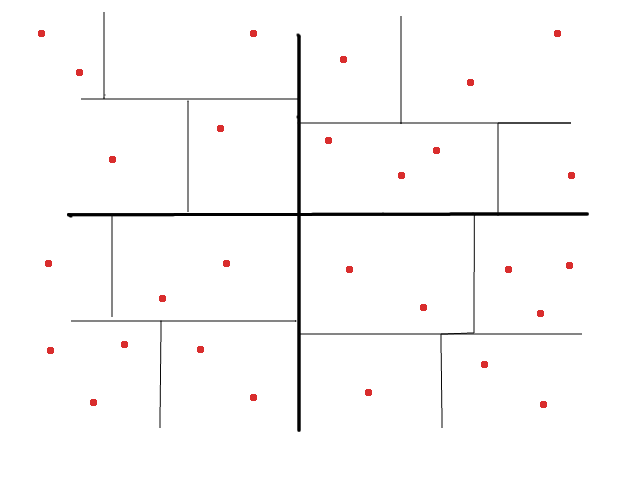
\includegraphics[width=8cm]{simple_boundary.png}%
  \caption{Storing whole area covered by nodes}
  \label{fig:covered}
\end{figure}
\pawel{Dałoby się zrobić te rysunki wektorowo?}

Imagine that we want to find point with smallest value of the $x$ coordinate. We need to process all nodes
that don't have a lower bound on $x$. Lets count them:
\bigskip

$T(1) = 1$

$T(n) \geq 2^{d-1} * T(n/2^{d})$

\bigskip

There are $\Omega (n^{1-1/d})$ such nodes. Instead of storing whole area covered by the node (see Figure~\ref{fig:covered}), we could calculate area covered by points inside node (Figure~\ref{fig:inside}).

\begin{figure}
\centering
  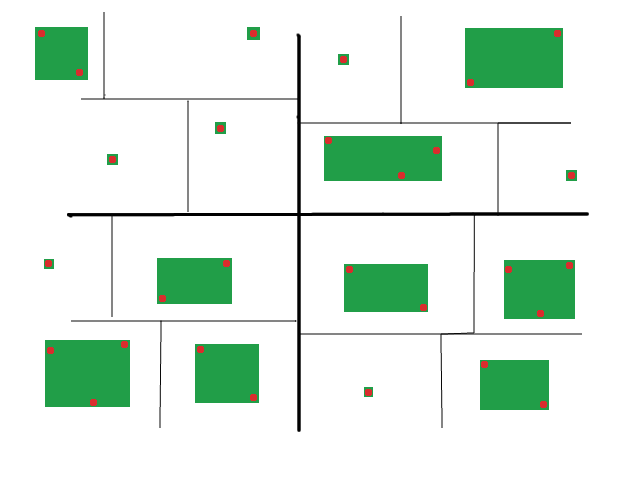
\includegraphics[width=8cm]{simple_boundary2.png}%
  \caption{Area covered by points inside nodes}
  \label{fig:inside}
\end{figure}

If values are unique, then there are only $\Oh(\log n)$ nodes with the minimal coordinate x (because there is only one such point, and it belongs to $\Oh(\log n)$ nodes). Therefore, using a priority queue implemented as a binary heap, complexity for such case would be $\Oh(\log n \log \log n)$. It can be improved by using binomial heaps \cite{BINOMHEAPS} . Binomial heap has an insert in amortized time of $\Oh(1)$ and finding minimum in $\Oh(1)$ which reduces complexity to $\Oh(\log n)$

\subsection{Raw pointers instead of boost::shared\textunderscore ptr}

In modern C++ pointers shouldn't be used, and shared pointers are recommended instead. Idea behind shared pointer is to automate releasing resources. Basically shared pointer keeps counter representing the number of copies of current pointer. When shared pointer is created, counter is incremented. When shared pointer is deleted, then counter is decremented. When counter is down to zero, then resource is released. With such a tool, developer is free from most common cause of memory leaks. Unfortunately such tool comes with time and space overhead. I decided to use raw pointers which give better running and space time.
Right now I think it was biggest mistake in the project. Source code became really messy, even small change in legacy code could create bugs.

\subsection{Balancing K-D tree}
K-D tree has similar problem to binary trees. Binary tree can be unbalanced and so can K-D tree. My idea for balancing K-D tree is very simple. When number of nodes in one subtree is 5 times larger that number of nodes in opposite subtree, then I'm rebuilding their parent subtree from the beginning.
This is the same idea which is used, for example, in the $\alpha$-balanced binary search trees \cite{ALPHATREES}. While the worst case complexity of a single operations can be large because of this rebalancing, the amortized complexity \cite{AMOR} is actually rather good.


\section{Complexities:}

Assumptions
\begin{enumerate}
\item All values of columns are different.
\item Rebuilding node causes number of nodes in one of its subtree to be not greater than twice the number of nodes in the opposite subtree.
\end{enumerate}

Let $n$ be number of points in the tree. Tree is somehow balanced so its height is $\Oh(\log n)$. Every point belongs to $\Oh(\log n)$ nodes. Let $|X|$ be number of points in subtree $X$.

\subsection{Inserting/deleting point $X$}
\begin{lemma}\label{lem:1}
Rebuilding tree of size S takes $\Oh(|S| \log |S|)$.
\end{lemma}

In linear time we can find median. After that we recursively rebuild two smaller subtrees. Complexity of such solution is $T(S) = 2 T(S/2) + \Oh(S)$ which is $T(S) = \Oh(|S| \log |S|).$

\begin{lemma}\label{lem:2}
Amortized time of insert/delete is $\Oh(\log^2 (n))$.
\end{lemma}

Consider that every node which is visited by insert/delete gets $\Oh(\log N)$ credits. By proving that each subtree has more credits than $|S| \log |S|)$ I will prove that amortized complexity of insert/delete is $\Oh(\log^2{N})$ .

There are two cases:
\begin{enumerate}
\item Subtree was never rebuild. Then this node has at least $10 |X| \log |X|$ credits. It is enough to rebuild subtree X.
\item Subtree was rebuild. Let $\xi$ be $|X|$ after last rebuild. Lets find smallest number of modifications required for another rebuild. We could either add points to larger subtree, or remove points from smaller subtree.
\begin{enumerate}
\item Inserting points to bigger subtree.

\begin{tabular}{|l|c|c|}
\hline  & Size of smaller subtree & Size of bigger subtree  \\
\hline Before & $x$ & $2x$ \\
\hline After & $x$ & $5x$ \\
\hline 
\end{tabular}

We need to insert at least $ \frac{5 - 2}{1 + 5} |S| = \frac{1}{2} |S|$ points to cause another rebuild. It means that at least $5 |S| \log |S|$ credits will be given which is enough. 

\bigskip
\item Deleting points from smaller subtree.

\begin{tabular}{|l|c|c|}
\hline  & Size of smaller subtree & Size of bigger subtree  \\
\hline Before & $5x$ & $10x$ \\
\hline After & $2x$ & $10x$ \\
\hline 
\end{tabular}

We need to delete at least $\frac{5 - 2}{2 + 10} |S| = \frac{3}{12} |S|$ points to cause another rebuild. It means that at least $\frac{5}{2} |S| \log |S|$ credits will be given which is enough. 

\end{enumerate}
\end{enumerate}

\subsection{Search}
Complexity of K-D tree doesn't change, it's still $\Oh(n^{1-1/d} + k)$. Lets remember that this complexity is worst case scenario. \jarek{Uważasz, że pisanie o average casie ma sens? Taki fragment jest przydany, ale bez względu na to jak go napiszę, brzmi jak wyciąganie królika z kapelusza;/} For average queries algorithm behaves like $\Oh(S \log n)$ where S = offset + limit. Explanation: when algorithm recursively enters node of K-D tree, then it usually finds some results. It means that finding single row, usually takes $\Oh(\log n)$.

\section{Tested engines}
\subsection{Solr}

Solr is a popular open source search platform from the Apache Lucene project. It has lots of very cool features like faceted searches, geospatial searches, string tokenizers (makes John and Johnny to be interpreted as the same name). It is easily extendable for new features. Solr implements master-slave replication which solves scalability problems. Everything is perfect except one thing. 

Solr doesn't modify database in real-time. Data isn't added immediately to database after insert/update commands. Data is actually inserted after calling commit command. Commit is very costly operation because it requires all caches to be invalidated. Even for table with few entries, commit takes more than 0.1 sec. Time for commit grows with growing size of data. Instance of Solr in nk contains 40 million entries and commit takes about 20 seconds. Commit doesn't block database which is very important. After commit, search engine is in warming stage. It means that all caches are deleted, so first queries can run slowly. After number of processed queries, engine is past warming stage and queries are handled much faster.

There is a rumour that twitter was able to modify source of Solr so they could have real-time modifications (apparently they succeeded, source needed).

Schema used in testing is:

\begin{lstlisting}
<fields>
  <field name="id" type="uuid" indexed="true" stored="true" default="NEW"/>
   <field name="first_name" type="text_general" indexed="true"
             stored="true" required="true" /> 
   <field name="last_name" type="text_general" indexed="true" 
             stored="true" required="true"/>
   <field name="age" type="int" indexed="true" stored="true" /> 
   <field name="city" type="text_general" indexed="true" stored="true"/>
</fields>

<uniqueKey>id</uniqueKey> 
\end{lstlisting}

Solr requires unique key. Combining all properties isn't enough. For example there are lots of guys named Jan Kowalski in Warsaw. Therefore I created another property named id.

\subsection{PostgreSQL}

PostgreSQL is very popular and the most trendy relational database nowadays. Defined requirements for this search engine are easily fulfilled by every relational databases. Only question is: How slow could it be ?

\begin{enumerate}
\item Prefix queries are handled by `property LIKE "text\%"`
\item Substring queries are handled by `property LIKE "\%text\%"`
\end{enumerate}

For text-search PostgreSQL implemented special type of indexes: GIN \cite{PSQLGIN} and GIST \cite{PSQLGIST}. Unfortunately I was unsuccessful in making them work with polish words. Therefore I'm testing PostgreSQL with default indexes.

\subsection{Sphinx search}

In nk we were really close to choosing Sphinx search over Solr. We didn't choose Sphinx because it dosn't have replication. It was the only reason. Replication is very important to us because in case of server failure we want to avoid downtime. I'm considering sphinx search in this paper because maybe some day they are going to implement some kind of replication.

For this problem real-time indexes are best \cite{SPHINXRT}.

\section{Tested results}

\subsection{How results are tested}

Testing environment is machine with Intel i5-2500 processor (4 cores, 3.5GHz), 8GB RAM and SSD drive. Comparing engines with default settings is pointless. I've tried to configure them all to production use. Most important change is increased memory limit to 2GB (it seems 25 percent RAM capacity is recommended limit for all engines).

In nk we've got several millions registered users. This number doesn't grow in spectacular fashion. I wan't to simulate engines behaviour in similar conditions. 

At the beginning I'm inserting $8 * 10^6$ random users. Then I'm running a script which creates random insert/search queries. It sends created queries for few hours and calculates statistics (avg running time, maximal running time).

Inserted data is generated in a very simple way. I've gather lists of most popular first names and last names in Poland (with counts). Probability of selecting name is proportional to it's count. Age is selected with linear distribution from set $[5, 100]$.

Search queries are generated by this procedure:
\begin{enumerate}
\item Pick N - number of expressions in search query
\item Column in expression is selected from set [first name, last name, age, city]. Each of them has 25 percent chance to be chosen.
\item If selected column has int type (only age is an integer) then possible queries are comparison and inequalities. There are 1 comparison and 4 inequalities. Each of them has 20 percent chance to be chosen.
\item If selected column has string type then possible queries are comparision, inequalities, prefix queries and substring queries. Each of them has $\frac{1}{7}$ chance to be chosen. Selected column is always compared to another string. This string is selected by selecting random word with 1-7 charactes. First character is uppercase others are lowercase characters. 
\end{enumerate}

Then I'm selecting random column and I'm setting it as order by column. Then I'm choosing offset and limit from range $[0, 20]$.

\subsection{Inserting 8 million rows}

8 million rows. Average string contains 7 characters. It means that size of inserted data is about 250 MB. There is always some overhead in keeping data structures. It causes shuffla to use 6 GB RAM.

It isn't most important part of testing. It is performed before production deployment and we are doing this part only once. I'm happy as long as indexing time doesn't last longer than a few hours. 

Shuffla inserts data with 1500 request per second. Using single inserts with other engines isn't so efficient. All considered engines are able to read csv file and import data from such file. This is fastest way to import data.

\todo{wykres z wynikami}

\subsection{Insert statistics}

\subsection{Search statistics}


\section{Summary}

\todo{tu troche napiszę}

%%%%%%%%%%%%%%%%%%%%%%%%%%%%%%%%%%%%%%%%%%%%%%%%%%

\begin{thebibliography}{99}

\bibitem{CGAAA} de Berg, Mark; Cheong, Otfried; van Kreveld, Marc; Overmars, Mark (2008). Computational Geometry 99-110

\bibitem{STUKK} E. Ukkonen. (1995). On-line construction of suffix trees. Algorithmica 14(3):249-260.

\bibitem{SOANS} http://stackoverflow.com/questions/10260688/boostproperty-treejson-parser-and-two-byte-wide-characters

\bibitem{REDPE} \url{http://redis.io/topics/persistence}

\bibitem{ASIOHTTP} \url{http://www.boost.org}

\bibitem{PSQLGIN} \url{http://www.sai.msu.su/~megera/wiki/Gin}

\bibitem{PSQLGIST} \url{http://www.postgresql.org/docs/9.1/static/gist-implementation.html}

\bibitem{PSQLINDEXES} \url{http://www.postgresql.org/docs/9.1/static/textsearch-indexes.html}

\bibitem{SPHINXRT} \url{http://sphinxsearch.com/docs/current.html#rt-indexes}

\bibitem{BINOMHEAPS}
Thomas H. Cormen, Charles E. Leiserson, Ronald L. Rivest, and Clifford Stein. Introduction to Algorithms, Second Edition. MIT Press and McGraw-Hill, 2001. ISBN 0-262-03293-7. Chapter 19: Binomial Heaps, pp.455–475.

\bibitem{ALPHATREES} Arne Andersson, Maintaining alpha-balanced Trees by Partial Rebuilding

\bibitem{AMOR} Robert Trajan, Amortized Computational Complexity

\end{thebibliography}

\end{document}


%%%%%%%%%%%%%%%%%%%%%%%%%%%%%%%%%%%%%%%%%%%%%%%%%%
